\documentclass{beamer}
\usepackage[utf8x]{inputenc}
\usepackage [T1]{fontenc}
\usepackage{beamerthemesplit} % new 
\usepackage{datetime}
\begin{document}
\title{Kompiuterinė rega. Automobilių numerių aptikimas.} 
\author{Motiejus Ėringis} 
\newdateformat{specialdate}{\THEYEAR-\twodigit{\THEMONTH}-\twodigit{\THEDAY}}
\date{\specialdate\today}

\frame{\titlepage} 

\frame{\frametitle{Turinys}\tableofcontents} 

\section{Trumpai apie OpenCV}
\frame{\frametitle{Trumpai apie OpenCV}
\begin{itemize}
\item Biblioteka apsimokančių algoritmų, skirtų vaizdų atpažinimui
\item<2-> Išleista 2000 m.
\item<3-> Atviro kodo ir nemokama
\item<4-> Programavimo sąsajos: C++, C, Python, Java, MATLAB/OCTAVE
\end{itemize} 
}

\section{Kas bus bandoma įgyvendinti}
\frame{\frametitle{Kas bus bandoma įgyvendinti}
\begin{itemize}
\item Lokalizuoti numerius
\item Apskaičiuoti transporto priemonės judėjimo greitį
\end{itemize} 
}

\section{Numerių lokalizavimas} 
\frame{\frametitle{Greičio apskaičiavimas} 
\begin{exampleblock}{Greičio formulė}
\begin{align*}
\overline{greitis}& = \frac{\Delta atstumas}{\Delta laikas}
\end{align*}
\end{exampleblock}
}

\begin{frame}
\frametitle{Numeriai}
520 mm x 110 mm
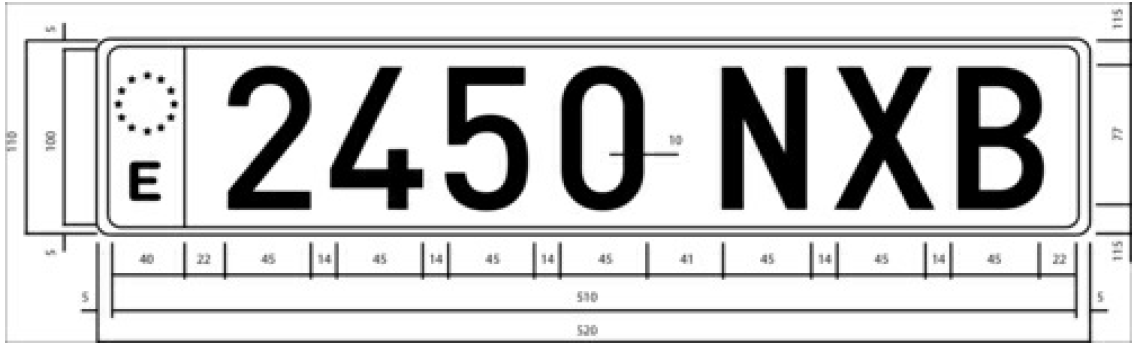
\includegraphics[scale=0.25]{numeriai.png}
\end{frame}

\begin{frame}
\frametitle{Atstumo nustatymas}
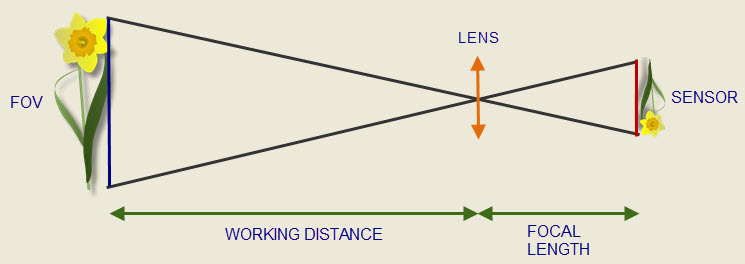
\includegraphics[scale=0.5]{lens.jpg}
\end{frame}

\frame{\frametitle{Atstumo nustatymas}
Žinomas numerių plotis D. Padarome nuotrauką su žinomu atstumu iki numerių Z. Išmatuojame numerių plotį gautais taškais - d. 
Židinio nuotolis:
\begin{align*}
 f &=\frac{d Z}{D}
\end{align*}
Pagal panašių trikampių sąvybę galime apskaičiuoti dabartinį atstumą Z' iki kameros:
\begin{align*}
Z'& = \frac{D' f}{d}
\end{align*}
}

\section{Numerių atpažinimas} 
\begin{frame}
\frametitle{Numerių atpažinimas}
\begin{itemize}
\item OpenCV biblioteka turi OCR funcijų, su kuriomis galima numerius atpažinti
\item<2-> Automatiniai vartai
\item<3-> Privalomojo draudimo tikrinimas
\item<4-> Nežymėtų patrulių aptikimas
\item<5-> Rinkliavų surinkimas
\end{itemize} 
\end{frame}


\section{Informacijos šaltiniai}
\frame{\frametitle{Informacijos šaltiniai}
\begin{itemize}
\item \url{http://www.regitra.lt/lt/transporto_priemoniu_registravimas/valstybinio_numerio_zenklai}
\item \url{https://en.wikipedia.org/wiki/OpenCV}
\item \url{http://www.cs.haifa.ac.il/~dkeren/ip/OReilly-LearningOpenCV.pdf}
\item \url{http://image2measure.net/files/Mastering_OpenCV.pdf}
\end{itemize} 
}

\end{document}



